\section{Paketverlust erkennen}
\label{sec:Paketverlust erkennen}

\subsection{ESP Aufbau}
\noindent Encapsulating Security Payload (ESP) wird bei IPsec (VPN) eingesetzt. Es gewährleistet die Vertraulichkeit und Integrität von Paketen und kümmert sich um die Authentisierung. Durch diese Integritätssicherung werden Pakete vor Manipulation geschützt.ESP verschlüsselt, im Unterschied zu Authentication Header (AH), die Nutzdaten. Bei AH werden nur die Integrität und Echtheit sichergestellt.

\noindent http://www.elektronik-kompendium.de/sites/net/1410261.htm

\noindent Der ESP header wird zwischen dem IP header und dem darunterliegenden Protokoll eingefügt (transport mode), oder es kapselt das ganze IP-Paket (tunnel mode).

\noindent RFC 2406

\noindent Der tunnel mode wird vor allem bei der Verbindung zwischen zwei Netzwerken über eine unsichere Verbindung eingesetzt. Der Modus unterstützt aber prinzipiell alle Arten von VPN-Anwendungen.Bei dieser Verwendung wird das ganze IP-Paket verschlüsselt und in ein neues IP-Paket verpackt. So wird das gesamte Paket durch ESP abgeschirmt und die eigentliche IP-Adresse des Absenders ist nicht mehr ersichtlich.Diese Methode hat natürlich einen gewissen Overhead. Es kommen 8 Byte für den ESP-Header, 16-20 Byte ESP-Trailer und für den neuen IP-Header 20 Byte hinzu.


\noindent Grafik für Tunnelmode
\noindent http://www.elektronik-kompendium.de/sites/net/1410261.htm

\noindent Bei einer Situation in der nur zwei Rechner miteinander verbunden werden, kann der Transportmodus verwendet werden. Dieser Modus unterstützt nur Host-to-Host Verbindungen. Da es für IPsec nicht unbedingt notwendig ist IP-Pakete vollständig neu zu enkapeln, können beim transport mode der originale IP-Header verwendet werden.Es kommen 8 Byte ESP-Header und 16-20Byte ESP-Trailer hinzu. Damit wird der Overhead kleiner, da man keinen zusätzlichen IP-Header benötigt.

\noindent Grafik für Transportmode

\noindent http://www.elektronik-kompendium.de/sites/net/1410261.htm

\noindent Wichtige Felder

\noindent Security Parameters Index (SPI) 32bits

\noindent Dieser willkürlich festgelegte Wert in Kombination mit der IP-Adresse des Ziels wird für eine Identifikation der Verbindung benötigt. Bei jeder neuen Verbindung wird die SPI neu gesetzt.

\noindent Sequence number 32bits

\noindent Die Sequence number wird für jedes Paket gesetzt und wird danach für jedes neue Paket um 1 erhöht. Bei einer neuen Verbindung wird die Sequece number stets auf 1 gesetzt.Falls Anti-Replay eingesetzt wird (standardmässig aktiviert) darf sich die Sequence number nicht wiederholen. Daher wird bevor das 2\^{}32 paket gesendet wird die Verbindung zurückgesetzt und eine neue SPI ausgehandelt. Damit wird auch die Sequence number wieder zurückgesetzt.

\noindent 


\subsection{Vorgehen bei Paketverlust}

{\raggedright
Falls ein \"{U}bertragungsmedium nicht korrekt funktioniert ist es m\"{o}glich,
dass Datenpakete nicht am Ziel ankommen oder mit einer zu grossen Versp\"{a}tung.
Da jedes \esp Paket mit einer Sequenznummer versehen ist, k\"{o}nnen diese
Paketverluste erkannt und gemeldet werden.
}

{\raggedright
Die \esp Pakete Besitzen zum Schutz vor Replay-Angriffen eine Sequenznummer sowie
einen bestimmten G\"{u}ltigkeitsbereich (Windowsize).
\\
Die Pakete k\"{o}nnen zum Beispiel durch Loadbalancing \"{u}ber unterschiedliche
Pfade verschickt werden. Dadurch kann die Reihenfolge der Pakete am Ziel nicht
mehr gew\"{a}hrleistet werden. Die zu sp\"{a}t ankommenden Pakete m\"{u}ssen
daher \"{u}berpr\"{u}ft werden, ob die Sequenznummer aktuell noch g\"{u}ltig ist
(innerhalb des Window).
}

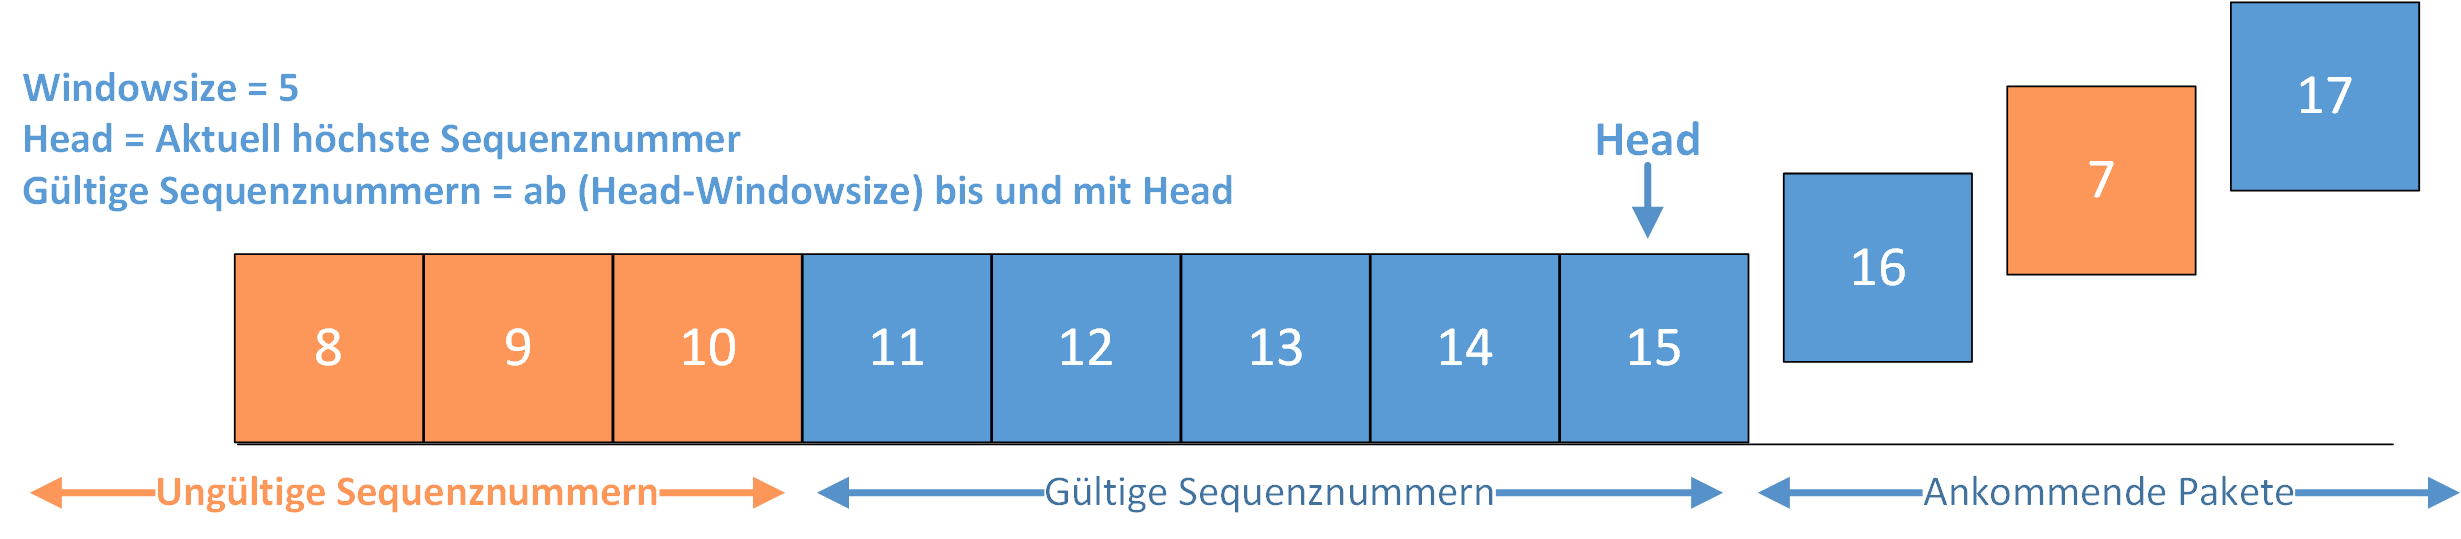
\includegraphics[width=1\textwidth]{start/img/Sequenznummern.png}

\subsection{Datenstruktur für die \esp Verbindungen}
Da pro Verbindung separate Sequenznummern verwendet werden, werden die verschiedenen Verbindungen durch eine Hashmap verwaltet. Als Key wird eine Struktur aus Source, Destination und \acs{SPI} verwendet. Als Value werden grundsätzlich zwei Listen für die Lost und MaybeLost Pakete benötigt. Zusätzlich wird noch ein Wert für den aktuellen Head gespeichert.

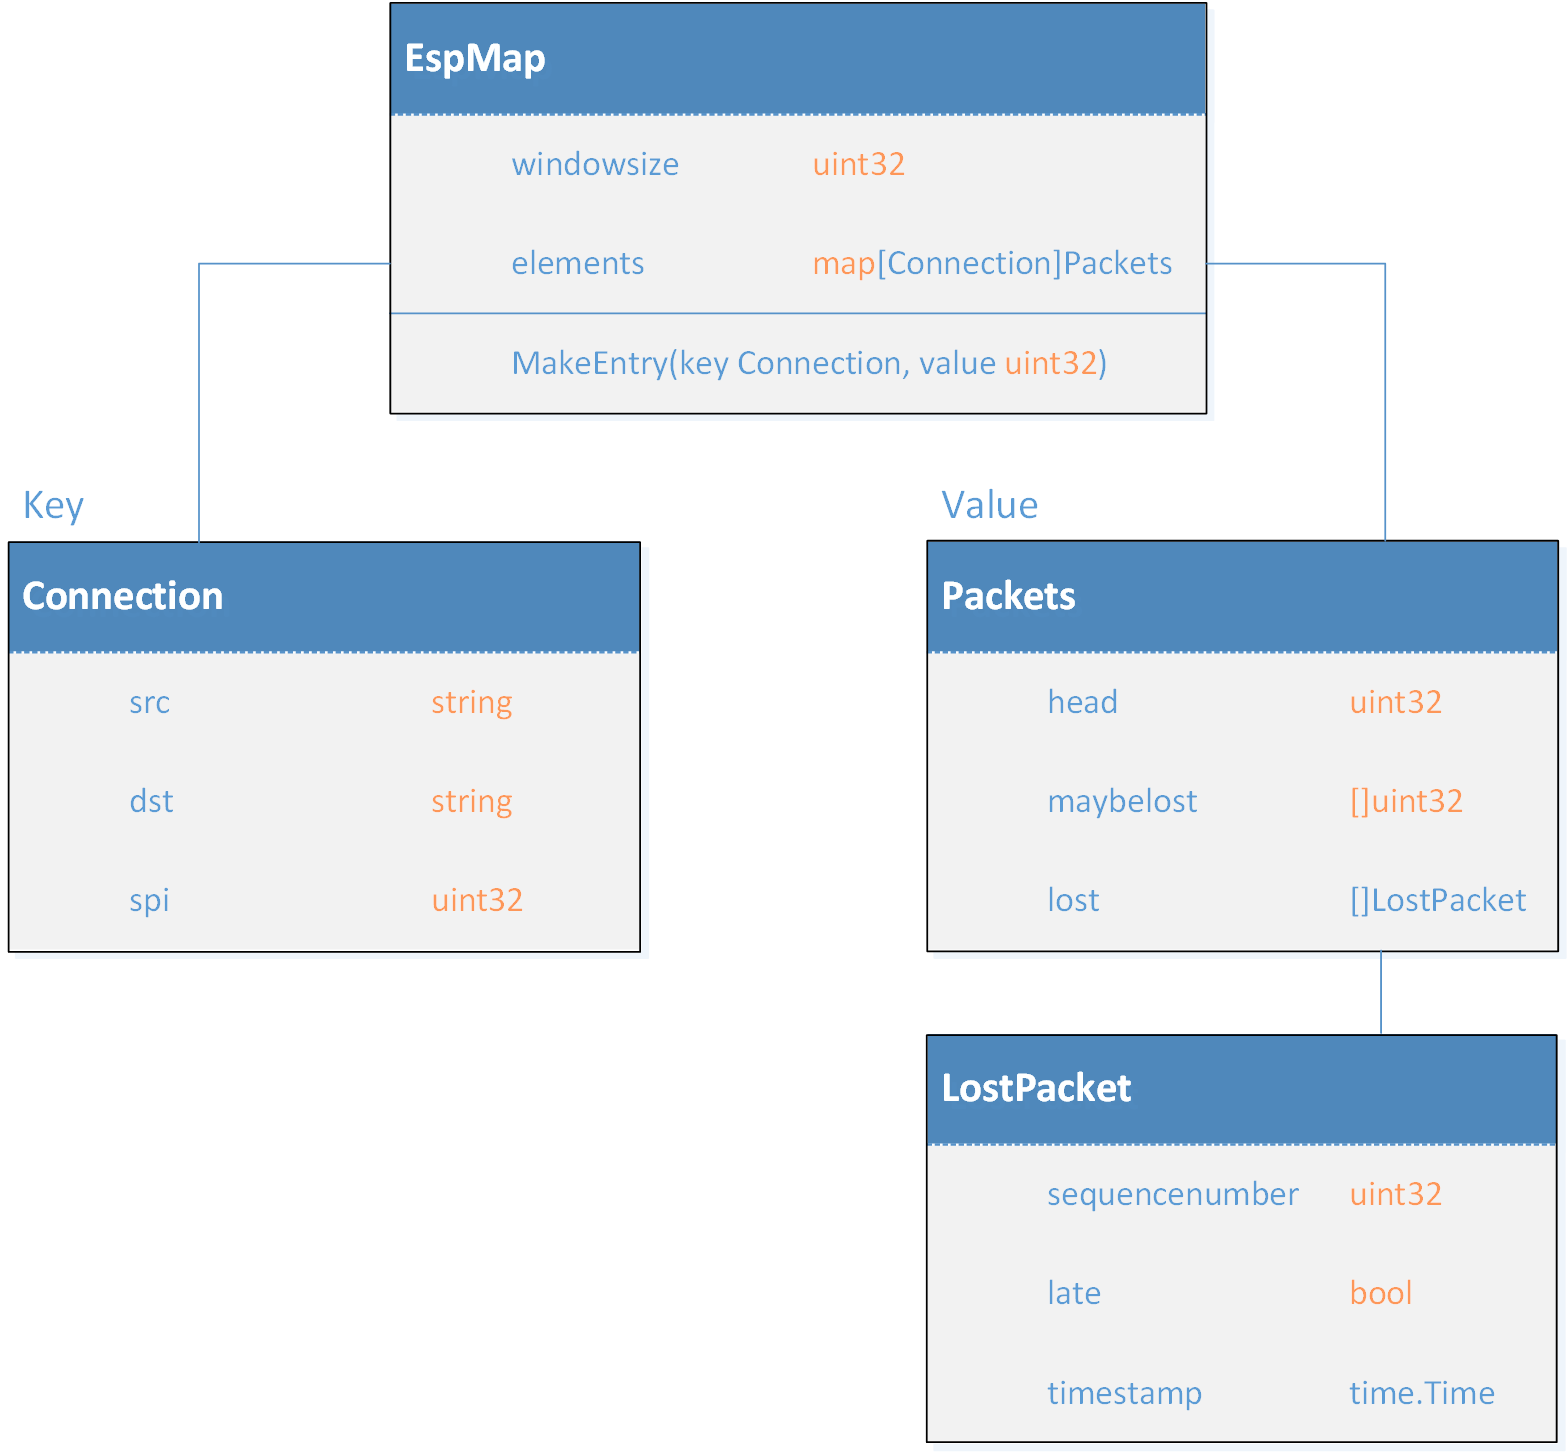
\includegraphics[width=1\textwidth]{start/img/Datenstruktur.png}

\subsection{Erkennung des Paketverlusts}
Die Paketverluste werden mit folgendem Algorithmus festgestellt.
Vereinfachte Darstellung des Algorithmus in Pseudocode:
\\
\textbf{Neues Packet Verarbeiten}
\begin{lstlisting}[language=go]
if(neuesPacket > Head){
	if(neuesPacket != Head + 1){
		Packete von Head bis neuesPacket in 
		MaybeLost speichern
	}
	Head = neuesPacket
	CheckLost()
}else{
	if(Head-WindowSize < neuesPacket){
		Packet aus MaybeLost entfernen
	}else{
		Flag fuer zu spaet angekommen setzen	
	}
}
\end{lstlisting}

\textbf{CheckLost}
\begin{lstlisting}[language=go]
for(MaybeLost){
	if(Head-WindowSize >= MaybeLostEintrag){
		Packet in Lost Speichern
		Packet aus MaybeLost entfernen
	}
}
\end{lstlisting}


\section{Syslogprotokoll}
\label{sec:Syslogprotokoll}

\noindent Syslog ist eines der am häufigsten eingesetzten Protokolle zum Übermitteln von Log-Meldungen in einem Netzwerk. Durch den einfachen Aufbau und die breite Unterstützung ist es leicht einsetzbar.


\subsection{ Aufbau}

\noindent Eine Syslog-Meldung besitzt ein Severity-Field womit der Schweregrad einer Nachricht festgelegt werden kann.

\noindent Die Werte besitzen folgende Bedeutungen:

\begin{tabular}{|p{0.5in}|p{3.7in}|} \hline 
Code & \textbf{Severity} \\ \hline 
0 & \textbf{Emergency:} system is unusable \\ \hline 
1 & \textbf{Alert:} action must be taken immediately \\ \hline 
2 & \textbf{Critical:} critical conditions \\ \hline 
3 & \textbf{Error:} error conditions \\ \hline 
4 & \textbf{Warning:} warning conditions \\ \hline 
5 & \textbf{Notice:} normal but significant condition \\ \hline 
6 & \textbf{Informational:} informational messages \\ \hline 
7 & \textbf{Debug:} debug-level messages \\ \hline 
\end{tabular}

RFC 5424

\noindent Zudem besteht eine Meldung noch aus einem Header sowie der eigentlichen Nachricht.

\noindent 


\section{ Meldungsaufbau}

\noindent Die Bedingungen für das Auslösen eines Alerts können im Configfile festgelegt werden. Es können der Zeitraum und die Anzahl Pakete definiert werden. Falls innerhalb dieses definierten Zeitraums die Anzahl an verlorenen Paketen überschritten wird, wird ein Alert ausgelöst.

\noindent Der Alert besitzt folgende Form:

\begin{tabular}{|p{0.5in}|p{0.7in}|p{3.0in}|} \hline 
Severity & Programm & Meldung \\ \hline 
1 & IpsecDiagTool & Too much LostPackets in Connection: (SPI: \dots ,SRC:\dots ,DST\dots ) \\ \hline 
\end{tabular}



\noindent So kann gleich anhand der Meldung erkannt werden um welche Verbindung es sich handelt und die notwendigen Schritte für eine Korrektur vorgenommen werden.

\noindent Damit es nicht zu einer Flut von Benachrichtigungen mit dem gleichen Inhalt und den gleichen Paketen kommt, wurde ein Timer von 10 Sekunden eingeführt.


\section{ Logging Package}

\noindent Das Logging wurde in einem separaten Package umgesetzt und stellt Methoden für das Logging zur verfügung. Das Package kapselt die benötigte Funktionalität die von „log/syslog`` benötigt wird.

\noindent Das Package wird vor Verwendung der Logging Funktionalität durch InitLogger initialisiert. Dabei werden die Werte für Zeitfenster, Anzahl Packete und Syslogserver gesetzt. Danach können die Benachrichtigungen mit AlertLog und InfoLog erstellt werden.

\noindent 


\section{ Benachrichtigung mit Datei}

\noindent Gleichzeitig mit dem Syslogeintrag wird eine CSV Datei erstellt. Die Datei Beinhaltet detaillierte Informationen um welche verlorenen Pakete es sich handelt und mit welchem Abstand ein Verlust detektiert wurde. Ausserdem gibt es Informationen ob ein Paket möglicherweise zu spät eingetroffen ist (also ausserhalb des Windows für die Sequenznummern). Falls dieses Problem vermehrt eintritt könnte ein erhöhen der Windowsize nötig sein.

\noindent Die Datei wurde so angepasst, dass sie mit Microsoft Excel oder ähnlichen Programmen problemlos gelesen und weiter verarbeitet werden kann.

\noindent 

\noindent Beispiel einer Datei

\begin{tabular}{|p{0.9in}|p{1.7in}|p{0.8in}|} \hline 
\multicolumn{2}{|p{1in}|}{SPI:12345 SRC: 192.168.0.1 DST: 192.168.0.2} &  \\ \hline 
Sequencenumber & Timestamp & ReceivedLater \\ \hline 
2 & Monday, 04-May-15 11:53:42 CEST & false \\ \hline 
3 & Monday, 04-May-15 11:53:42 CEST & true \\ \hline 
4 & Monday, 04-May-15 11:53:42 CEST & false \\ \hline 
5 & Monday, 04-May-15 11:53:42 CEST & false \\ \hline 
\end{tabular}



\noindent 
